% Format teze zasnovan je na paketu memoir
% http://tug.ctan.org/macros/latex/contrib/memoir/memman.pdf ili
% http://texdoc.net/texmf-dist/doc/latex/memoir/memman.pdf
% 
% Prilikom zadavanja klase memoir, navedenim opcijama se podešava 
% veličina slova (12pt) i jednostrano štampanje (oneside).
% Ove parametre možete menjati samo ako pravite nezvanične verzije
% mastera za privatnu upotrebu (na primer, u b5 varijanti ima smisla 
% smanjiti 
\documentclass[11pt,oneside]{memoir}

% Paket koji definiše sve specifičnosti mastera Matematičkog fakulteta
\usepackage{matfmaster}
\usepackage{amsmath}
\usepackage{float}

\DeclareMathOperator*{\argmax}{arg\,max}
\DeclareMathOperator*{\argmin}{arg\,min}
%
% Podrazumevano pismo je ćirilica.
%   Ako koristite pdflatex, a ne xetex, sav latinički tekst na srpskom jeziku
%   treba biti okružen sa \lat{...} ili \begin{latinica}...\end{latinica}.
%
% Opicija [latinica]:
%   ako želite da pišete latiniciom, dodajte opciju "latinica" tj.
%   prethodni paket uključite pomoću: \usepackage[latinica]{matfmaster}.
%   Ako koristite pdflatex, a ne xetex, sav ćirilički tekst treba biti
%   okružen sa \cir{...} ili \begin{cirilica}...\end{cirilica}.
%
% Opcija [biblatex]:
%   ako želite da koristite reference na više jezika i umesto paketa
%   bibtex da koristite BibLaTeX/Biber, dodajte opciju "biblatex" tj.
%   prethodni paket uključite pomoću: \usepackage[biblatex]{matfmaster}
%
% Opcija [b5paper]:
%   ako želite da napravite verziju teze u manjem (b5) formatu, navedite
%   opciju "b5paper", tj. prethodni paket uključite pomoću: 
%   \usepackage[b5paper]{matfmaster}. Tada ima smisla razmisliti o promeni
%   veličine slova (izmenom opcije 12pt na 11pt u \documentclass{memoir}).
%
% Naravno, opcije je moguće kombinovati.
% Npr. \usepackage[b5paper,biblatex]{matfmaster}

% Pomoćni paket koji generiše nasumičan tekst u kojem se javljaju sva slova
% azbuke (nema potrebe koristiti ovo u pravim disertacijama)
\usepackage{pangrami}

% Paket koji obezbeđuje ispravni prikaz ćiriličkih italik slova kada
% se koristi pdflatex. Zakomentarisati ako na sistemu koji koristite ovaj
% paket nije dostupan ili ako ne radi ispravno.
\usepackage{cmsrb}

% Ostali paketi koji se koriste u dokumentu
\usepackage{listings} % listing programskog koda
\usepackage{hyperref}

% Ime kandidata na srpskom jeziku (u odabranom pismu)
\autor{Момир Аџемовић}
% Naslov teze na srpskom jeziku (u odabranom pismu)
\naslov{Предикциjа траjекториjа више обjеката на сцени}
% Godina u kojoj je teza predana komisiji
\godina{2022}
% Ime i afilijacija mentora (u odabranom pismu)
\mentor{др Младен Николић, ванредни професор\\ Универзитет у Београду, Математички факултет}
% Ime i afilijacija prvog člana komisije (u odabranom pismu)
\komisijaA{др Јована Ковачевић, доцент\\ Универзитет у Београду, Математички факултет}
% Ime i afilijacija drugog člana komisije (u odabranom pismu)
\komisijaB{др Александар Картељ, доцент\\ Универзитет у Београду, Математички факултет}
% Ime i afilijacija trećeg člana komisije (opciono)
% \komisijaC{}
% Ime i afilijacija četvrtog člana komisije (opciono)
% \komisijaD{}
% Datum odbrane (obrisati ili iskomentarisati narednu liniju ako datum odbrane nije poznat)
\datumodbrane{15. септембар 2022.}

% Apstrakt na srpskom jeziku (u odabranom pismu)
\apstr{%
У изради...
}

% Ključne reči na srpskom jeziku (u odabranom pismu)
\kljucnereci{машинско учење, аутономна вожња, растеризација, графовске неуронске мреже}

\begin{document}
% ==============================================================================
% Uvodni deo teze
\frontmatter
% ==============================================================================
% Naslovna strana
\naslovna
% Strana sa podacima o mentoru i članovima komisije
\komisija
% Strana sa posvetom (u odabranom pismu)
\posveta{посвета... у изради...}
% Strana sa podacima o disertaciji na srpskom jeziku
\apstrakt
% Sadržaj teze
\tableofcontents*

% ==============================================================================
% Glavni deo teze
\mainmatter
% ==============================================================================

% ------------------------------------------------------------------------------
\chapter{Увод}
% ------------------------------------------------------------------------------

Аутономна вожња подразумева потпуну или парцијалну аутоматизацију процеса контроле возила коришћењем рачунарских и осталих технологија. Агент (возило) 
у овом случају мора да има способност опажања окружења и самосталног кретања кроз то окружење ради остваривања задатог циља 
(краткорочно: паркирање, скретање, ... дугорочно: транспорт, ...). Кључне
компоненте које се интегришу у овај систем су:
\begin{itemize} 
  \item Детекција и праћење објеката у околини (опажање окружења са акцентом на покретне објекте) 
  \item Разумевање њихових циљева, како би се сам циљ агента ускладио са њима (први корак за омогућавање самосталног кретања кроз окружење).
\end{itemize} 
Прва компонента се реализује помоћу специјалних сензора као што су \textit{LiDAR} сензори за конструкцију 3D мапе окружења, \textit{Radar} сензора
за детекцију удаљености и брзине објеката (погодан и у случају лошег времена) и камере који прикупљају 2D слике окружења. Саме камере помоћу
метода машинског учења могу да извршавају исте послове као и радари (као што то човек ради користећи само вид). Циљ овог рада се односи на други део
тј. анализа постојећих радова чија је тама разумевање циљева објеката на сцене где се агент налази. Будуће трајекторије тих објеката се посматрају
као циљеви, а сама трајекторија агента се усклађује у односу на њих.

\section{Аутономна вожња}

Министарство саобраћаја САД и NHTSA (\textit{National Highway Traffic Safety Administration}) је усвојила \textit{Society of Automotive Engineers (SAE)}
стандард који прописује 6 нивоа аутоматизације од нултог, где човек има потпуну контролу до петог, где рачунар самостално управља возилом:\cite{ad_survey}
\begin{itemize}
  \item \textbf{Ниво 0}: Човек има потпуну контролу над возилом
    \begin{itemize}
      \item Возило може да има једноставније аутоматизације као што је на пример аутоматизовано кочење у хитним случајевима.
    \end{itemize}
  \item \textbf{Ниво 1}: Човек и рачунар сарађују у процесу управљања возилом (сва одговорност је на возачу).
  \item \textbf{Ниво 2}: Рачунар има потпуну контролу, али човек мора да буде присутан и да реагује у било ком тренутку ако је то неопходно (сва одговорност је на возачу).
  \item \textbf{Ниво 3}: Рачунар има потпуну контролу ако су испуњени одређени услови, а човек је у том случају потпуно ослобођен свих дужности вожње. 
    \begin{itemize}
      \item Ако услови више не важе (нпр. пада снег), онда човек мора да преузме одговорност над возилом.
      \item Када су испуњени услови, одговорност је на произвођачу софтвера за аутономну вожњу.
    \end{itemize}
  \item  \textbf{Ниво 4}: Слично као ниво 3, али возило је испрограмирано тако да се само заустави у случају да услови нису испуњени.
    \begin{itemize}
      \item Када сви услови опет важе, возило-рачунар може да настави да врши свој задатак.
    \end{itemize}
  \item  \textbf{Ниво 5}: Рачунар има потпуну контролу над возилом у сваком тренутну.
\end{itemize}

\section{Поставка проблема}

Предвиђање трајекторија или предвиђање кретања једног агента на сцени са више покретних објеката (суседи аналогни агенту) се формално
дефинише као предикција скупа вредности $\{(x^{t}_a, y^{t}_a)\ |\ t \in [0, T]\}$, где је $T$ дужина трајекторије агента која се предвиђа, 
под претпоставком да су дате следеће информације:
\begin{itemize}
  \item Историја тог агента $A_{h} = \{(x^{t}_a, y^{t}_a)\ |\ t \in [-H, -1]\}$, где је $H$ дужина историје трајекторије;
  \item Историја осталих покретних агената $\{T^{n}_{raj}\ |\ n \in N\}$, где је $T^{n}_{raj}$ истог облика као и $A_{h}$, а $N$ је скуп
        свих суседа;
  \item Окружење агента $E$ - варира у односу на скуп података (путеви, пешачки прелази, семафори, ...).
\end{itemize}

Сам проблем је општији од примене у аутономног вожњи (предвиђање кретања пешака), али представља кључну компоненту у системима за
аутономну вожњу.

\section{\textit{HD} мапе}

Мапа са високим нивоом детаља (\textit{eng. HD map}) је мапа путева са прецизношћу до пар центиметара и високим нивоом
познавања окружења: позиције пешачких прелаза, позиције семафора, полигони путева, смерови улица итд... Битно је нагласити
да су \textit{HD} мапе супериорне у односу на \textit{GPS} у смислу прецизности и разноврсности информација. Саме \textit{GPS}
мапе нису довољно прецизне да може да их користи систем за аутономну вожњу уместо људи који су значајно робуснији на грешке
\textit{GPS}-a (што може да буде и до неколико метара). Аналогија HD мапа са човеком и вожња добро познатим путем и вожња 
непознатим путем први пут у животу. Вожња добро познатим путем одговара знању које се добија из HD мапа. 


Овај тип података даје јако велику количину информација које се могу процесирати у целокупном систему аутономне вожње. Два главна проблема
и изазова овог типа података је њихово прикупљање (LiDAR системи су скупи) и одржавање, и обрада овако неструктуираних података. Алтернатива
је коришћење камера и модела дубоког учења за прикупљање података о окружењу у реалном времену.

\begin{figure}[H]
  \centering
  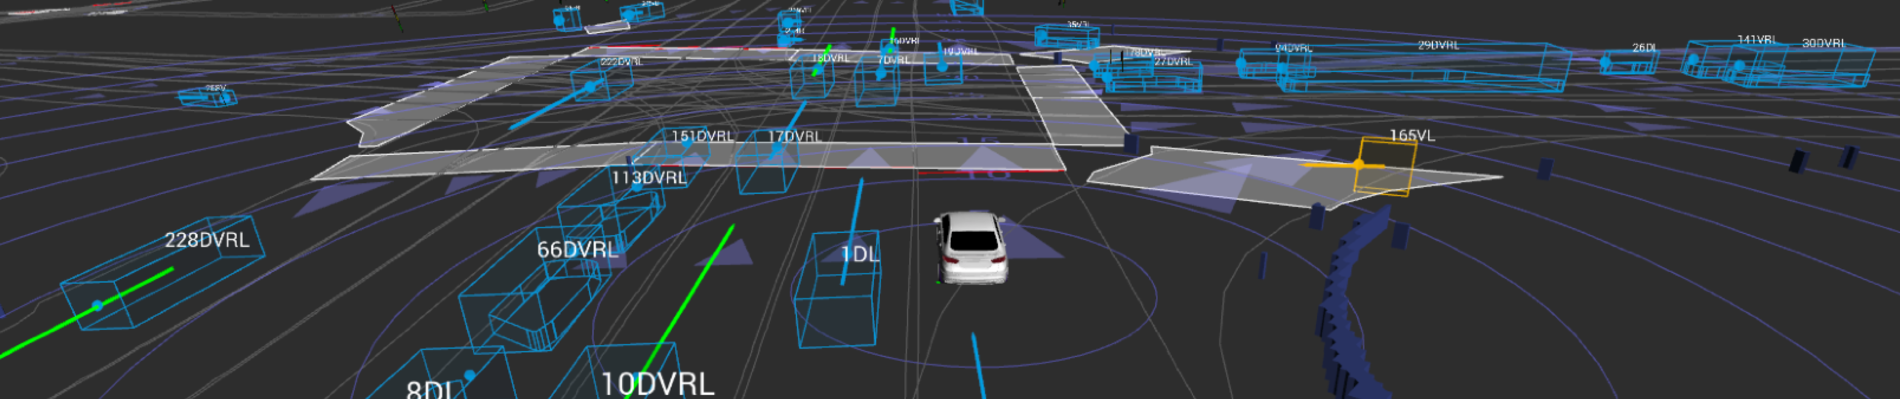
\includegraphics[width=0.9\textwidth]{images/lyft-hd-map.png}
  \caption{\textit{HD} мапа - \textit{Kaggle Lyft} \cite{kaggle_lyft} \label{kaggle-lyft-example}}
\end{figure}

На слици \ref{kaggle-lyft-example} се види пример визуализоване \textit{HD} мапе. Бело возило је агент, а плави правоугаоници су суседи. 
Са слике се види да мапе садрже и полигоне пешачких прелаза и још неке додатне податке. Подаци ових мапа су често у \textit{3D} формату
тј. узима се у обзир и висина. У реалном времену се ови подаци могу комбиновати са улазима из камера. 

\chapter{Преглед основних градивних елемената}
\label{chp:razrada}

\section{Неуронске мреже}

TODO: Osnovno, MLP

\section{Конволутивне неуронске мреже}

TODO: Mozda se i ne budu koriscene

\section{Графовске неуронске мреже}

TODO: Osnovno, opšte, GCN, GraphSage

\section{Механизам пажње}

TODO: attention

\chapter{Преглед претходних приступа}
\label{chp:razrada}
% ------------------------------------------------------------------------------

Техника за предикцију трајекторија више објеката које издвајају посебан објекат као агент, могу да се групишу грубо у четири групе:
\begin{itemize}
  \item Технике прилагођене репрезентацијама временских серија;
  \item Технике засноване на растеризацији;
  \item Технике засноване на графовским репрезентацијама;
  \item Хибридне технике.
\end{itemize}
Постоје и општије технике које не разликују конкретно агента од осталих објеката у процесу предвиђања.

\section{Технике прилагођене репрезентацијама временских серија}

Група модела која је интуитивна као иницијални приступ овом проблему који се своди на предвиђање временских серија, јесу рекурентне неуронске мреже 
(\textit{eng. RNN - Recurrent neural network}) и конволутивне мреже за једну димензију (\textit{CNN - Convolutional Neural Network}). 
Често коришћена \textit{LSTM} архитектура рекурентних неуронских мрежа погодна за кодирање динамике објеката. 
Како трајекторија једног објекта зависи од трајекторија осталих објеката,
неопходно је да се користи механизам пажње као компонента модела која учи везе између различитих објеката на сцени. \cite{argoverse} \cite{social_lstm} 
Мана овог скупа модела је што модели нису погодни за потпуно разумевање контекста сцене (објекти, возне линије, саобраћајни знакови, ...). Такође,
једна од главних проблема оваквих директних приступа је неспособност модела да научи мултимодалну природу трајекторија на сцени.

Уместо учења модела који дају предикције трајекторија које се у просеку најбоље у тим случајевима (проблем мултимодалности), 
алтернатива су скуп архитектура заснованих на (условљеним) генеративним моделима који
омогућавају генерисање произвољног броја трајекторија кроз узорковање из условљене расподеле (расподела је условљена историјом трајекторије, као и
окружењем у којем се тај објекат налази). Пример је \textit{Social GAN} \cite{social_gan} архитектура која узима у обзир претходне наведене услове и генерише 
,,социјално прихватљиве`` трајекторије пешака. 
У случају возила са агентом, генеративни модели захтевају током процеса предикције напредније алгоритме узорковања ради оптимизације покривености
трајекторијама\footnote{Покривеност се односи на метрике које узимају у обзир више од једне трајекторије, па је битно и да те
саме трајекторије буду разноврсне}.

\section{Технике засноване на растеризацији}

Растеризација подразумева трансформацију \textit{HD} мапа у формат слике, где слике приказују сцене из птичје 
перспективе (\textit{eng. BEV - Bird's-eye-view}).
Предност овог формата је могућност учења контекста тих мапа коришћењем више слојева конволутивних неуронских мрежа.
Овакве компоненте архитектуре (низ повезаних конволутивних мрежа од улаза) се често називају енкодери\footnote{Сам појам енкодера није везан само 
за појам конволутивних слојева, већ било које слојееве}. 
Конволутивне мреже нису ограничене да раде са RGB и сличним форматима слика тј. сваком пикселу може да се додели низ својстава. 
Нека од очигледнијих својстава су: да ли агент заузима тај пиксел, да ли сусед (неагент) заузима тај пиксел,
да ли пиксел припада улици, ... Излаз CNN енкодера се углавном накнадно комбинује са осталим компонентама за генерисање резултата. 

Излази модела такође могу да се представљају као слике тј. топлотне мапе \textit{(eng. Heat Map)}, где се сваком пикселу додељује вероватноћа
да се агент (или посматрани објекат) налази на тој локацији. Топлотне мапе се добијају декодерима који комплементирају енкодер компоненте.
То значи да није неопходно да се експлицитно постави ограничење на одређени број излазних трајекторија модела. Проблем
код више излазних трајекторија модела је то што може да изазове колапс моде (eng. \textit{mode collapse}). Број трајекторија се овде не 
дефинише експлицитно и може да варира од једне сцене до друге. Наравно, не узимају се сви пиксели као кандидати, већ се примењује неки
алгоритам узорковања. Алгоритам узорковања у том случају даје флексибилност, где може сам алгоритам да се имплементира тако
да је најпогоднији за неку од метрика тј. даје боље резултате за једну метрику у односу на остале. \cite{home} \cite{centernet} 

Архитектура \textit{HOME} \cite{home} користи овај принцим за паралелно кодирање растеризоване сцене и трајекторија oбјеката. Резултати
компоненти се спајају и прослеђују као улаз у декодер за генерисање топлотне мапе. Узорковањем тачака из топлотних мапа се добија скуп кандидата тачака.
Главна претпоставка архитектура заснованих на топлотним мапама је: Ако знамо циљну тачку и историју трајекторије објекта, онда можемо
једноставно да одредимо трајекторију до те циљне тачке\footnote{Ова претпоставка је такође основа за многе друге методе}. 
За одређивање ових трајекторија могу да се користе једноставнији модели неуронских мрежа (нпр. потпуно повезане мреже).

Могуће је растеризовати потпуно податке тј. растеризовати и трајекторије као низ слика. Свака слика садржи скуп тачака које представљају
локације објеката. Архитектура \textit{CASPNet} \cite{caspnet} примењује CNN енкодер на свако стање и користи ConvLSTM \cite{convlstm} за разумевање
темпоралних веза. На овај начин се извлаче својства динамичког дела сцена. На сличан начин је могуће и извући својства и за 
статички део (возне линије, возни површине, ...) користећи класичне конволутивне мреже. Комбинацијом ових података се генеришу
трајекторије које су исто у растеризованом облику.

\section{Технике засноване на графовским репрезентацијама}

Мапе имају комплексну топологију. Технике засноване на растеризацији користе конволуцију која тешко 
извлачи потпуно семантику тих мапа, а такође су конволуције скупе операције. Алтернатива је моделовање мапа графовским структурама. 
Технике засноване на графовском репрезентацијом као улаз добијају стање мапе кодиране као граф и примењују моделе графовских неуронских мрежа. 
Две архитектуре које представљају основе за већину архитектура ове групе су \textit{LaneGCN} \cite{lanegcn} и \textit{VectorNet} \cite{vectornet}.

Мапа може да се моделује као скуп повезаних сложених линија (\textit{end. polylines}), где сваком објекту одговара једна усмерена сложена линија. 
\textit{VectorNet} је хијерархијска графовска неуронска мрежа која као улаз добија мапу која је моделована као скуп 
сложених линија, а као резултат даје скуп предикција трајекторија. Идеја је да се прво извуку својста из сложених 
линија појединачних објеката, а онда то пронађу одговарајуће међусобне везе између објеката и везе између објеката и возних линија. 
За проналазак међусобних веза се користи механизам пажње. \cite{attention_is_all_you_need} \cite{vectornet} 

Архитектура \textit{LaneGCN} нуди варијанту конволутивних графовских мрежа (\textit{GCN - Graph Convolution Network}) 
која је специјализована за графове путних линија које имају различите типове веза. Користе се различите матрице
повезаности за суседе, претходнике, следбенике (леви и десни) у контексту путева. За сваку матрицу повезаности може да се примени класичан GCN, а
комбиновањем тих елемената је добија један \textit{LaneGCN} слој. \cite{lanegcn} Сам модел се своди на \textit{GCN} са више матрица повезаности.

\section{Хибридне технике}

Хибридне технике користе комбинацију структура графова и BEV слика. \textit{GOHOME} Модификована верзија \textit{HOME} која уместо
CNN енкодера и растеризованих слика мапа, користи \textit{LaneGCN} архитектуру за енкодер. Заправо ансамбл ова два модела (\textit{HOME, GOOME})
даје најбоље резултате по \textit{MR} метрици\footnote{Објашњење за ову метрике се налази у секцији за евалуацију}.

\section{Технике засноване на облацима тачака}

Последња група нешто одступа од осталих али и даље даје добре резултате. Подаци се посматрају као облаци тачака (\textit{eng. point cloud}) 
и примењују се технике намењене за такву структуру података. Основна
архитектура је \textit{TPCN} \cite{tpcn} која је заснована на \textit{PointNet} \cite{pointnet}, а већина осталих техника су ,,изведене``.

% ------------------------------------------------------------------------------
% ------------------------------------------------------------------------------

\chapter{Метрике за евалуацију модела}
\label{chp:razrada}
% ------------------------------------------------------------------------------

Неке од стандардних метрика за евалуацију квалитета предикције трајекторија су ,,просечнa грешка одступања`` (\textit{eng. ADE - Average Displacement Error})
и ,,последња грешка одступања`` (\textit{eng. FDE - Final Displacement Error}). У наставку се користе енглеске скраћенице \textit{ADE} и
\textit{FDE}. Метрика \textit{ADE} се добија
упросечавањем еуклидског растојања између временски синхронизованих тачака трајекторија предикције и реализације. 
Метрика \textit{FDE} узима у обзир само последњу тачку тј. еуклидско растојање између последње тачке реализације и предикције. 
\cite{social_gan} \cite{argoverse} 
У наставку се налазе формуле у случају да се посматра тачно један објекат (нпр. само агент):

\begin{figure}[H]
  \centering
  $ADE = \frac{1}{T}\sum_{k=1}^{T}\sqrt{(x_k - \hat{x}_k)^2 + (y_k - \hat{y}_k)^2}$
\end{figure}

\begin{figure}[H]
  \centering
  $FDE = \sqrt{(x_{last} - \hat{x}_{last})^2 + (y_{last} - \hat{y}_{last})^2}$
\end{figure}

Метрике се једноставно уопштавају у случајевима где постоји више објеката на сцени:

\begin{figure}[H]
  \centering
  $ADE = \frac{1}{T\times N}\sum_{n=1}^{N}\sum_{k=1}^{T}\sqrt{(x^n_k - \hat{x}^n_k)^2 + (y^n_k - \hat{y}^n_k)^2}$
\end{figure}

\begin{figure}[H]
  \centering
  $FDE = \frac{1}{N}\sum_{n=1}^{N}\sqrt{(x^n_{last} - \hat{x}^n_{last})^2 + (y^n_{last} - \hat{y}^n_{last})^2}$
\end{figure}

Ако узмемо у обзир претпоставку да се релативно детерминистичкi може da se одреди трајекторија ако је дата њена последња тачка 
(што је у случају возила разумна претпоставка), онда су ове две метрике корелисане у смислу да модел који има добар \textit{FDE}, има и добар \textit{ADE}
(и супротно).

Ове једноставне метрике су погодне када претпостављамо да је расподела трајекторија унимодална тј. да је природа трајекторија претежно детерминистичка. 
Скупови података трајекторија могу да имају јачу стохастичку природу због стохастичке природе самих објеката (трајекторија) или непотпуних опажања окружења
(непотпуне информације). 
Пример таквог скупа података је скуп трајекторија пешака. Пешак који је прешао пешачки прелаз, може у том тренутку да скрене лево или десно.
У том случају имају два вероватна сценарија за исту историју трајекторије (углавном немамо информације о циљевима самог пешака). \cite{social_gan} \cite{best_of_many_cvae}
У случају возила је ситуација мало блажа због претходне претпоставке, али и даље је тешко одредити крајњу тачку трајекторије која може значајно да варира 
(да ли вожач жели да скрене десно или иде право, да ли вози брже или спорије, ...). 

Скуп ,,најбољи из групе`` (\textit{eng. ,,Best of Many``}) техника узимају у обзир мултимодалну природу расподела трајекторија. Модел може
да генерише неколико различитих предикција трајекторија и за сваку трајекторију да да одговарајућу вероватноћу (поузданост). Као грешка се узима предикција
која је најбоља по дефинисаном критеријуму (критеријум не мора да се поклапа са самом мером која се користи). \cite{best_of_many_cvae} \cite{argoverse}
Претходно наведене технике \textit{ADE} и \textit{FDE} се уопштавају у \textit{minADE} и \textit{minFDE}. Због једноставности узимају се у обзир облици
са једним објектом: \cite{Disdis} \cite{best_of_many_cvae}

\begin{figure}[H]
  \centering
  $minADE = ADE(\displaystyle\argmin_{\hat{T}^k_{raj}} FDE(\hat{T}^k_{raj}, T_{raj}), T_{raj}), k \in \{1, ..., K\}$ 
\end{figure}

\begin{figure}[H]
  \centering
  $minFDE = \displaystyle\min FDE(\hat{T}^k_{raj}, T_{raj}), k \in \{1, ..., K\}$
\end{figure}

Уколико модел генерише више од \textit{K} трајекторија, узима се и обзир првих \textit{K} по поузданости. У специјалном случају када је $K = 1$, онда 
\textit{minFDE} постаје \textit{FDE}, а \textit{minADE} се и даље разликује по избору ,,главне`` трајекторије. 
Проблем са \textit{minADE} i \textit{minFDE} је у томе што не узимају у обзир остале трајекторије поред најбоље и самим тим се не прави разлика
између предикције са свим добрим трајекторијама и предикције са једном добром трајекторијом. \cite{Disdis} 
Друга замерка овим метрикама је што не узимају у обзир поузданост предикција након филтрирања \textit{K} трајекторија. Уколико је најбоља трајекторија
прецизна, желимо и даље да знамо да ли је модел сигуран или је добар резултат последица ,,среће``. Модификоване метрике: \cite{home}

\begin{figure}[H]
  \centering
  $p\mbox{--}minADE = ADE(\hat{T}^{min}_{traj}, T_{raj}) - \ln{P(\hat{T}^{min}_{traj}|E_{nv})}$
\end{figure}

\begin{figure}[H]
  \centering
  $p\mbox{--}minFDE_{prob} = FDE(\hat{T}^{min}_{traj}, T_{raj}) - \ln{P(\hat{T}^{min}_{traj}|E_{nv})}$
\end{figure}

Овде је $\hat{T}^{min}_{traj}$ трајекторија која има најбољу $FDE$ оцену, а $p(\hat{T}^{min}_{traj}|E_{nv})$ је условљена вероватноћа те 
трајекторије $\hat{T}^{min}_{traj}$ у односу на стање окружења $E_{nv}$. Уколико је мала грешка по метрици \textit{ADE} (\textit{FDE}) за одговарајућу трајекторију, 
али њена одговарајућа вероватноћа има малу вредност, онда негативан логаритам те вероватноће има велику вредност. 
\cite{argoverse} У импементацији се ова вероватноћа ограничава са доње стране, како не
би дошло до прекорачења због велике апсолутне вредности након примене логаритма на веома мале вредности.

Уместо упросечавања \textit{L2} растојања у сваком кораку, могу да се броје кораци у којима трајекторије одступају за више од $MR_{thresh}$. 
Мотивација за ову метрику је чињеница да одступање које је 1 или 2 метра од реализације није толико релевантно у односу на 
велику разлику одступања. \cite{home} Такође постоји верзија метрике која узима у обзир вероватноћу и кажњава предикцију 
модела ако је добра, а модел је ипак несигуран.

\begin{figure}[H]
  \centering
  $MR = \sum^T_{k=1} I(||\hat{T}^{k}_{traj} - T_{raj}||_{2} \geq MR_{thresh})$
\end{figure}

\begin{figure}[H]
  \centering
  $MR_{prob} = \sum^T_{k=1} I(||\hat{T}^{k}_{traj} - T_{raj}||_{2} \geq MR_{thresh}) $
  $+ I(||\hat{T}^{k}_{traj} - T_{raj}||_{2} < MR_{thresh}) \cdot (1.0 - P(\hat{T}^{k}_{traj}|E_{nv}))$
\end{figure}

\noindent У случају \textit{Argoverse} скупа података, за параметар $MR_{thresh}$ се узима 4 пиксела тј. 2 метра у реалном свету. 

Све до сада наведене метрике су опште примене на било које објекте за које се предвиђају трајекторије. Пошто је агент углавном возило, може да
се анализира да ли предвиђена трајекторија скреће са пута. Због тога се уводи метрика ,,сагланост са продучјем вожње`` 
(\textit{eng. DAC - Drivable Area Compilance}), која одређује учесталост трајекторија које нису скренуле са пута од изабраних 
\textit{K} трајекторија: \cite{argoverse}

\begin{figure}[H]
  \centering
  $DAC = \frac{DAC_{occurences}}{T}$
\end{figure}

У евалуацији модела се узимају у обзир све метрике. За параметар \textit{K} се узима вредност 6.

\chapter{Припрема података}

Основни скуп података за тренирање и тестирање техника предикције трајекторија је \textit{Argoverse Motion Forecasting} скуп података
који се састоји од 324 хиљаде детаљних мапа саобраћаја (\textit{eng. ,,HD maps``}) које садрже геометријске и семантичке податке сцена. Постоје две \textit{HD} сцене
за градове Питсбург и у Мајами. Коришћењем аутономних возила су генерисани сценарији који представљају неколико узастопних слика сцена (у табеларном формату)
на деловима мапа. Сви детаљи о овом скупу података се могу пронаћи на адреси 
\href{https://www.argoverse.org/index.html}{\color{blue}{www.argoverse.org}} \cite{argoverse}. \\


\noindent Kључне информације које се издвајају из сваког сценарију су:
\begin{itemize}
  \item Мапа сценарија (Питсбург или Мајами);
  \item Трајекторије агената;
  \item Трајекторије осталих објеката на сцени;
  \item Путеви - возне (централне) линије.
\end{itemize}

\section{Претпроцесирање података}

Подаци сваког сценарија се векторизују и чувају у полу-структуираном формату. 
За парсирање и обраду улазних података се користи \textit{argoverse API} интерфејс. Циљ овог корака процесирања података
је векторизација података и релативно је независан од модела који се користи.

Трајекторија агента\footnote{Низ $(x, y)$ тачака, где је приближна временска разлика између две тачке око 0.1 секунде у \textit{Argoverse}
скупу података} 
се дели на два дела: историја (својства) и реализација (будуће вредности). Реализација се састоји од $N_r$ 
опажања $x$ и $y$ координата тј. облик реализације је $(N_r, 2)$.. 
Историја се аналогно формира да садржи историју $N_h$ опажања $x$ i $y$ релативних координата. Овај део трајекторије иде непосредно
пре реализације. Посматрамо следеће случајеве:
\begin{itemize}
  \item Постоји више од $N_h + N_r$ опажања: Одбацује се реп трајекторије (првих неколико вредности хронолошки гледано);
  \item Постоји мање од $N_{hmin} + N_r$ опажања: Сценарио се одбацује (сматра се да је невалидан);
  \item Постоји између $N_{hmin} + N_r$ и $N_h + N_r$ опажања: реп трајекторије се допуњава до димензије $N_h + N_r$ 
  посматрано као да објекат мирује у тим тренуцима.
\end{itemize}
Коначно, облик историје је $(N_h, 3)$, где трећа вредност означава да ли је опажање право ($1$) или допуњено ($0$).

Све координате се нормализују тако да су релативне у односу на последње опажање у трајекторији историје агента. Последње опажање историје
агента има координату (0, 0) у новом координатном систему, а све остале тачке се транслирају за вектор $-C$, где је $C$ оригинална позиција
последњег опажања. Координатни систем се такође ротира тако да се вектор који је одређен првом и последњом тачком историје трајекторије 
(поједностављен правац трајекторије) поклапа са \textit{y}-осом сличко као и у оригиналном \textit{Vectornet} раду \cite{vectornet}. Последња
трансформација је скалирање свих координата са $\frac{1}{25}$, где је ова вредност добијена анализом стандардних девијација свих тачака
на сценаријима (узета је просечна вредност свих сценарија). Ове трансформације су кључне за перформансе модела, јер је сам проблем који се решава
једноставнији:
\begin{itemize}
  \item Применом транслације модел не мора да учи где се агент налази, јер је то увек (0, 0) координата;
  \item Применом ротације моделу је олакшано учење усмерења трајекторије тј. моделу је лакше да одреди оријентацију агента;
  \item Применом скалирања се добијају стабилнији градијенти.
\end{itemize}


Трајекторије суседних објеката се деле на два дела аналогно трајекторији агента. Неопходно је да се синхронизују трајекторије 
суседних објеката по временским ознакама (eng. \textit{timestamp}) са трајекторијом агента, јер не постоји у сваком тренутку исти
број објеката на сцени. Након синхронизације се трајекторије деле на историју и реализацију и проверава се да ли дужине тих
делова задовољавају критеријуме:
\begin{itemize}
  \item Уколико је дужина трајекторије историје краћа од $N_{homin}$, онда се објекат одбацује;
  \item Уколико је дужина трајекторије реализације краћа од $N_{romin}$, онда се објекат исто одбацује.
\end{itemize}

Као додатна провера, за сваки сусед се провера растојање од агента. Уколико је сусед превише далеко, онда се се он одбацује.
Критеријум за одбацивање суседа узима у обзир брзину агента (по $x$ и $y$ оси одвојено) и растојање њихових последњих опажања
у трајекторији историје. Уколико неки од следећих услова није
испуњен, онда се сусед игнорише у сценарију: 
\begin{itemize}
  \item $\frac{O_n^x}{V_s^x} \leq T_{steps}$
  \item $\frac{O_n^y}{V_s^y} \leq T_{steps}$
\end{itemize}
где је $O_n^x$ ($O_n^y$) нормализована $x$ ($y$) координата суседа, $V_s^x$ ($V_s^y$) је наивно 
апроксимирана\footnote{Брзина се апроксимира као просек промена координата у трајекторији историје} брзина агента
по $x$ ($y$) оси и $T_{steps}$ је параметар толеранције.
Трајекторије се секу или допуњавају до фиксног облика (kao што је то у случају припреме трајекторије агента). 
Векторизован облик: $(N_n, N_h, 3)$ за историје трајекторија и $(N_n, N_r, 3)$ за реализацију трајекторија, где је $N_n$ број судедних објеката. 

На основу локације агента се издвајају сегменти путева (централне линије - возне путање) који нису даље од агента за више од $D_{lsinit}$. Уколико нема
пронађених сегмената централних линија, онда се вредност за $D_{lsinit}$ множи $K_{ls}$\footnote{$D_{lsinit}$ и $K_{ls}$ су фиксне вредности
у \textit{argoverse} интерфејсу} пута до највише $D_{lsmax}$ (ако и даље нема сегмената, 
онда се сценарио одбацује, јер није пронађен ниједан путни сегмент у околини). 
За сваки сегмент се чува низ од 20 $(x, y)$ координата приширених са метаподацима:
\begin{itemize} 
  \item \textit{is\_intersection} - да ли се сегмент сече са неким сегментом,
  \item \textit{turn\_right} - да ли је у питању скретање у десно, 
  \item \textit{turn\_left} - да ли је у питању скретање у лево, 
  \item \textit{turn\_none} - да ли нема стретања, 
  \item \textit{is\_traffic\_control} - да ли постоји контрола саобраћаја. 
\end{itemize}
Коначан облик је $(N_{ls}, 20, 7)$. 

Постоји коначан број путних сегмената по којој
објекат може да се креће у скоријој будућности на задатој мапи, због чега је корисно да се информације о кандидатима путних сегмената
користе као улаз у модел или као хеуристике.
Основа алгоритма за проналазак ових кандидата се налази у \textit{argoverse} интерфејсу. Кандидати се проналазе једноставним
алгоритмом који подразумева проналажење најближег путног сегмента последњем опажању трајекторије агента. Тај путни
сегмент представља почетни чвор за примену обиласка графа путних сегмената у дубину (\textit{eng. Depth-First Search - DFS}). 
Довољно је да се пронађу суседи у том графу који су довољно близу самом агенту (следбеници). \cite{argoverse}
Овај алгоритам не даје оптималне резултате и постоји доста простора за унапређење. 


Коначан векторизован облик је: $(N_c, N_r, 3)$, где је $N_c$ број пронађених кандидата,
$N_r$ дужина трајекторије реализације. Пошто се путеви допуњавају по потреби до димензије $N_r$, користи се трећа координата
за маску. На табели \ref{dp-params-table} се види преглед свих параметара процеса.

\begin{table}
  \begin{tabular}{c|c}
    Ознака параметра & Објашњење \\
    \hline
    $N_r$ & Дужина трајекторије реализације (део који се предвиђа) \\
    $N_h$ & Дужина трајекторија историје \\
    $N_{hmin}$ & Минимална дужина трајекторије историје пре допуњавања \\
    $N_{hоmin}$ & Минимална дужина трајекторије историје суседа пре допуњавања \\
    $N_{rоmin}$ & Минимална дужина трајекторије реализације суседа пре допуњавања \\
    $T_{steps}$ & Умножак максималног растојања до сегмента пута \\
    $D_{lsmax}$ & Максимално растојање до пута
  \end{tabular}
  \caption{Преглед параметара припреме података}
  \label{dp-params-table}
\end{table}

На сликама \ref{scenario-example-148229} и \ref{scenario-example-16518} се налазе примери два визуализована сценарија
након претходне припреме. У овом формату нису прикази делови сцене на којој је могућа вожња, али 
постоје више путања по којим возила могу да се крећу са истом историјијом трајекторије (зависно од циља). 
Изузеци су у случају неких скретања, промени линија, ...

\begin{figure}[H]
  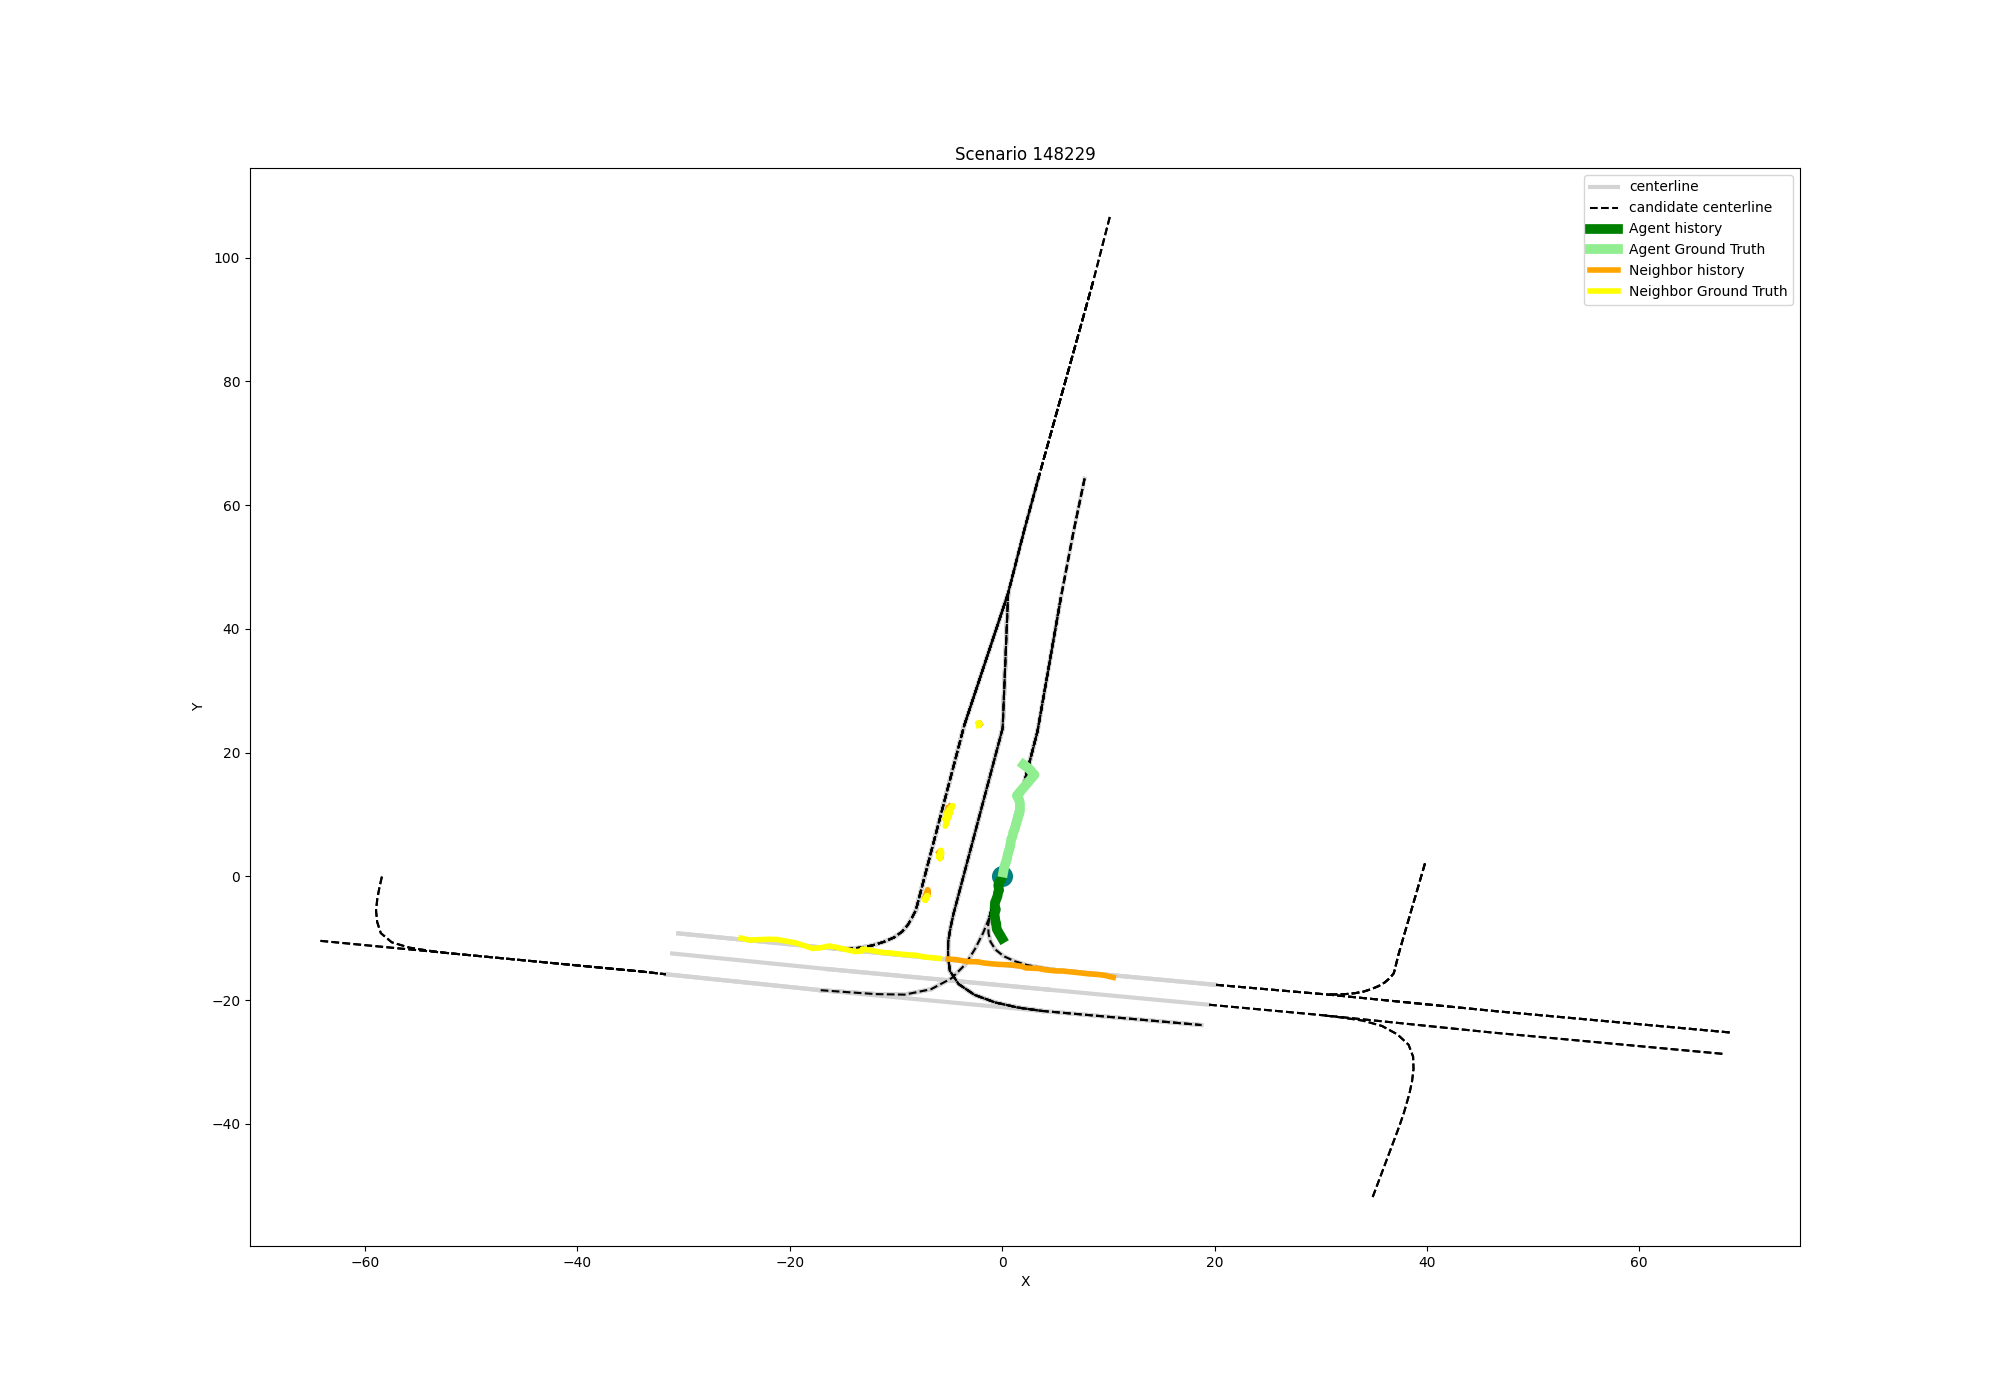
\includegraphics[width=0.9\textwidth]{images/scenario_148229.png}
  \caption{Визуализација припремљених података - Пример 1}
  \label{scenario-example-148229}
\end{figure}

\begin{figure}[H]
  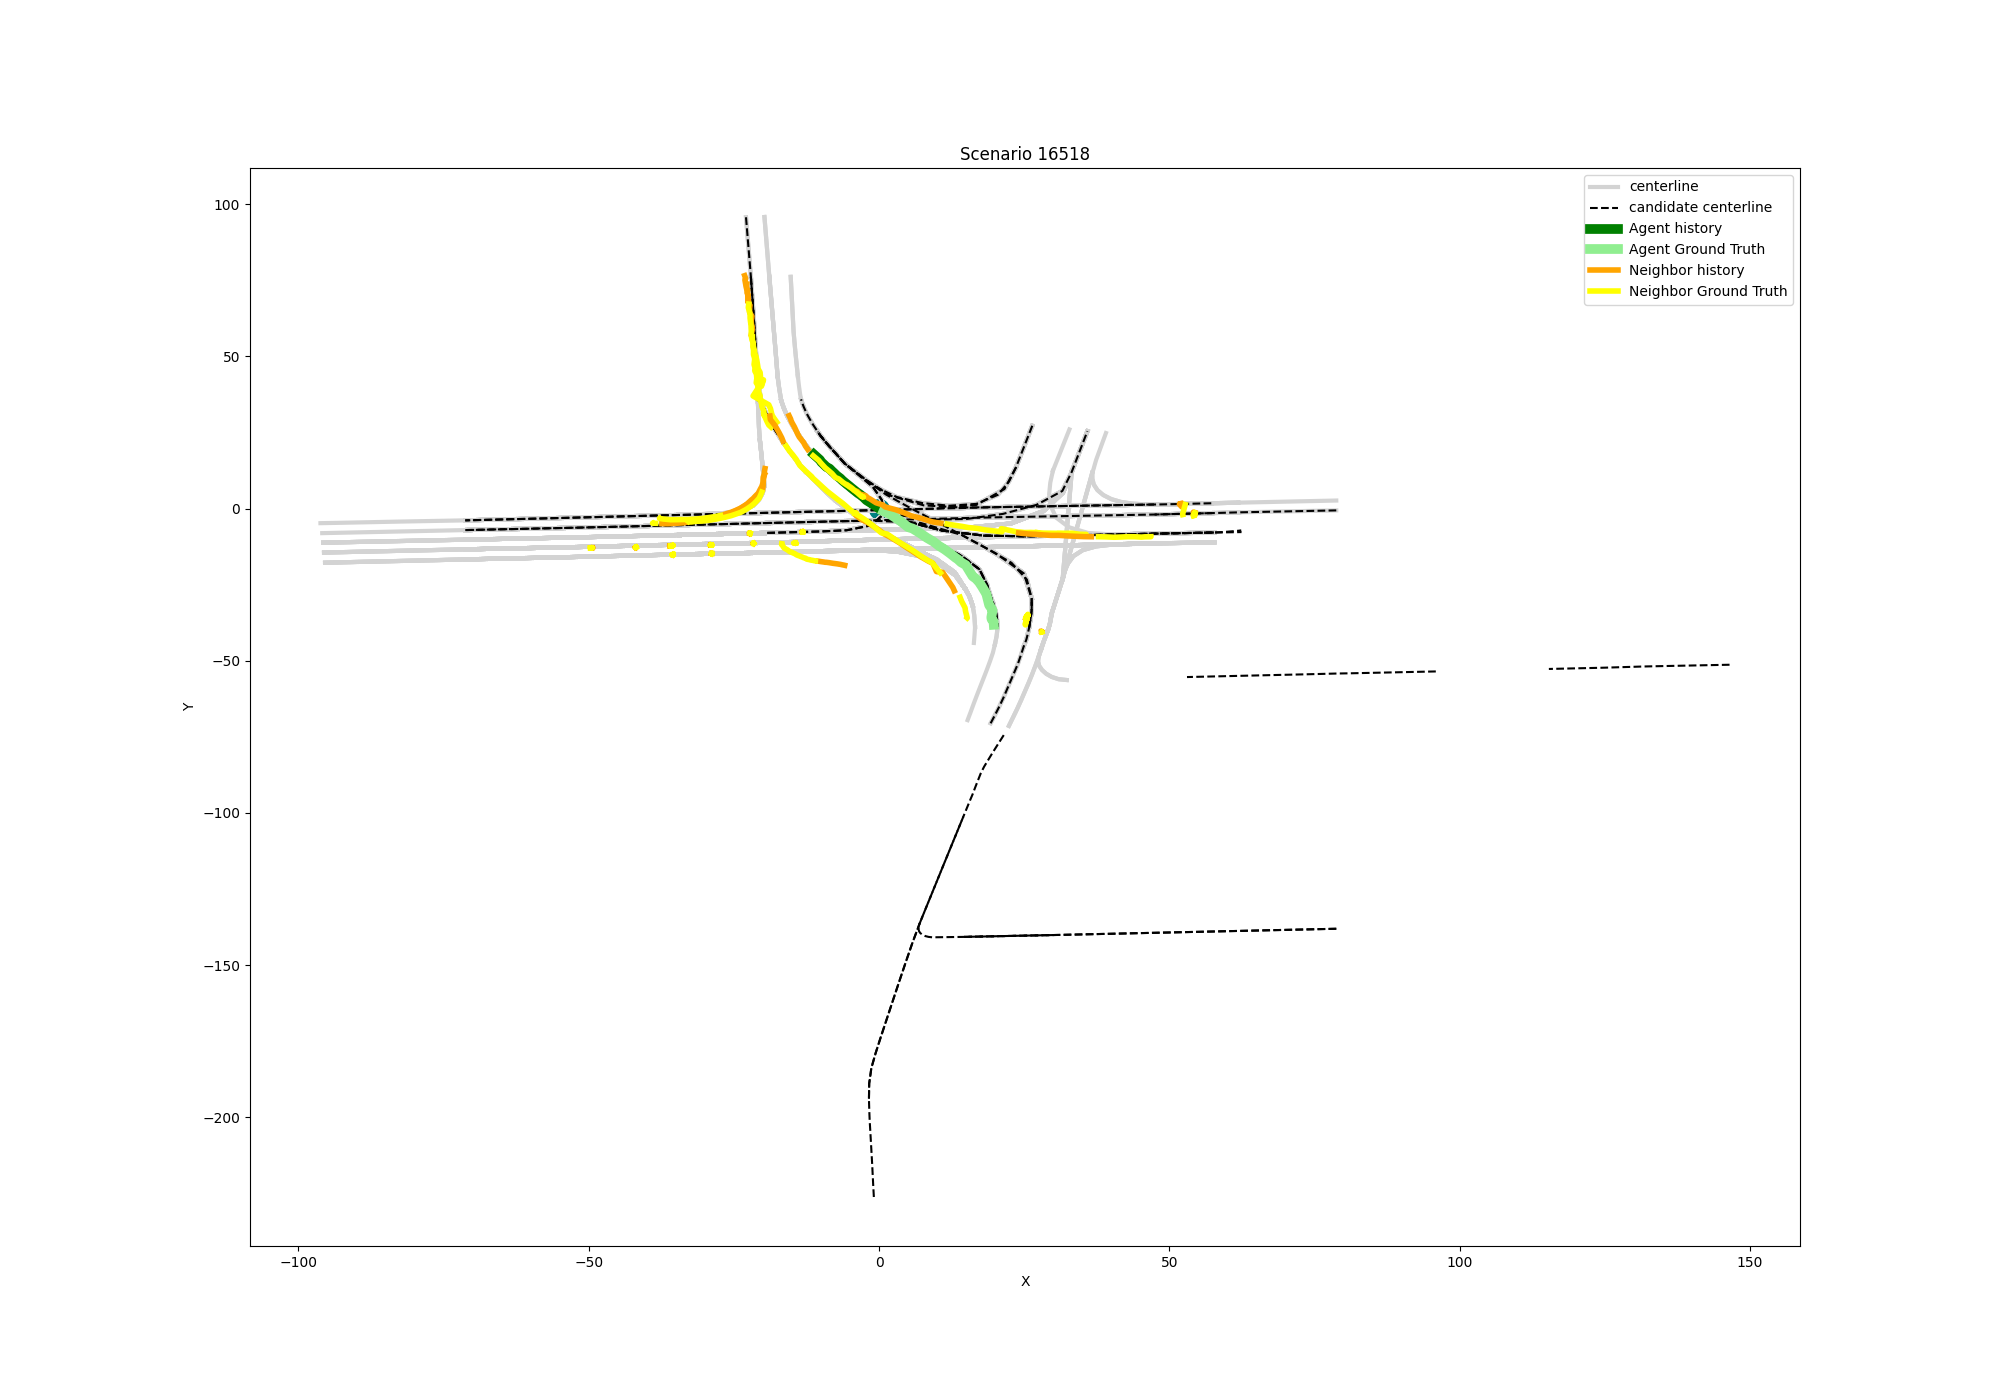
\includegraphics[width=0.9\textwidth]{images/scenario_16518.png}
  \caption{Визуализација припремљених података - Пример 2}
  \label{scenario-example-16518}
\end{figure}

% ------------------------------------------------------------------------------
\chapter{Техника заснована на разумевању контекста обрадом сцене представљене графом}
\label{chp:razrada}
% ------------------------------------------------------------------------------

Независно од конкретног скупа података \textit{HD} мапа, сваки сценарио може да се представи графовском структуром која повезује тачке на сцени, где
свака тачка има своја својства:
\begin{itemize}
  \item Трајекторија агента и објеката је скуп тачака усмереног графа - сложена незатворена линија (\textit{eng. polyline}) (сваки чвор је повезан са следећим).
  \item Путеви могу да се представе на исти начин као и објекти, али разлика је у самим својствима чворова помоћу којих се путеви 
        разликују од објеката.
  \item Пешачки прелаз је полигон, који може да се представи као сложена затворена линија. 
\end{itemize}

Овакав приступ представљања сцена на апстрактном нивоу је лако прилагодљив било ком скупу података. Начин даље трансформације компоненти овог графа
зависи од самог модела. \cite{vectornet}

\begin{figure}[H]
  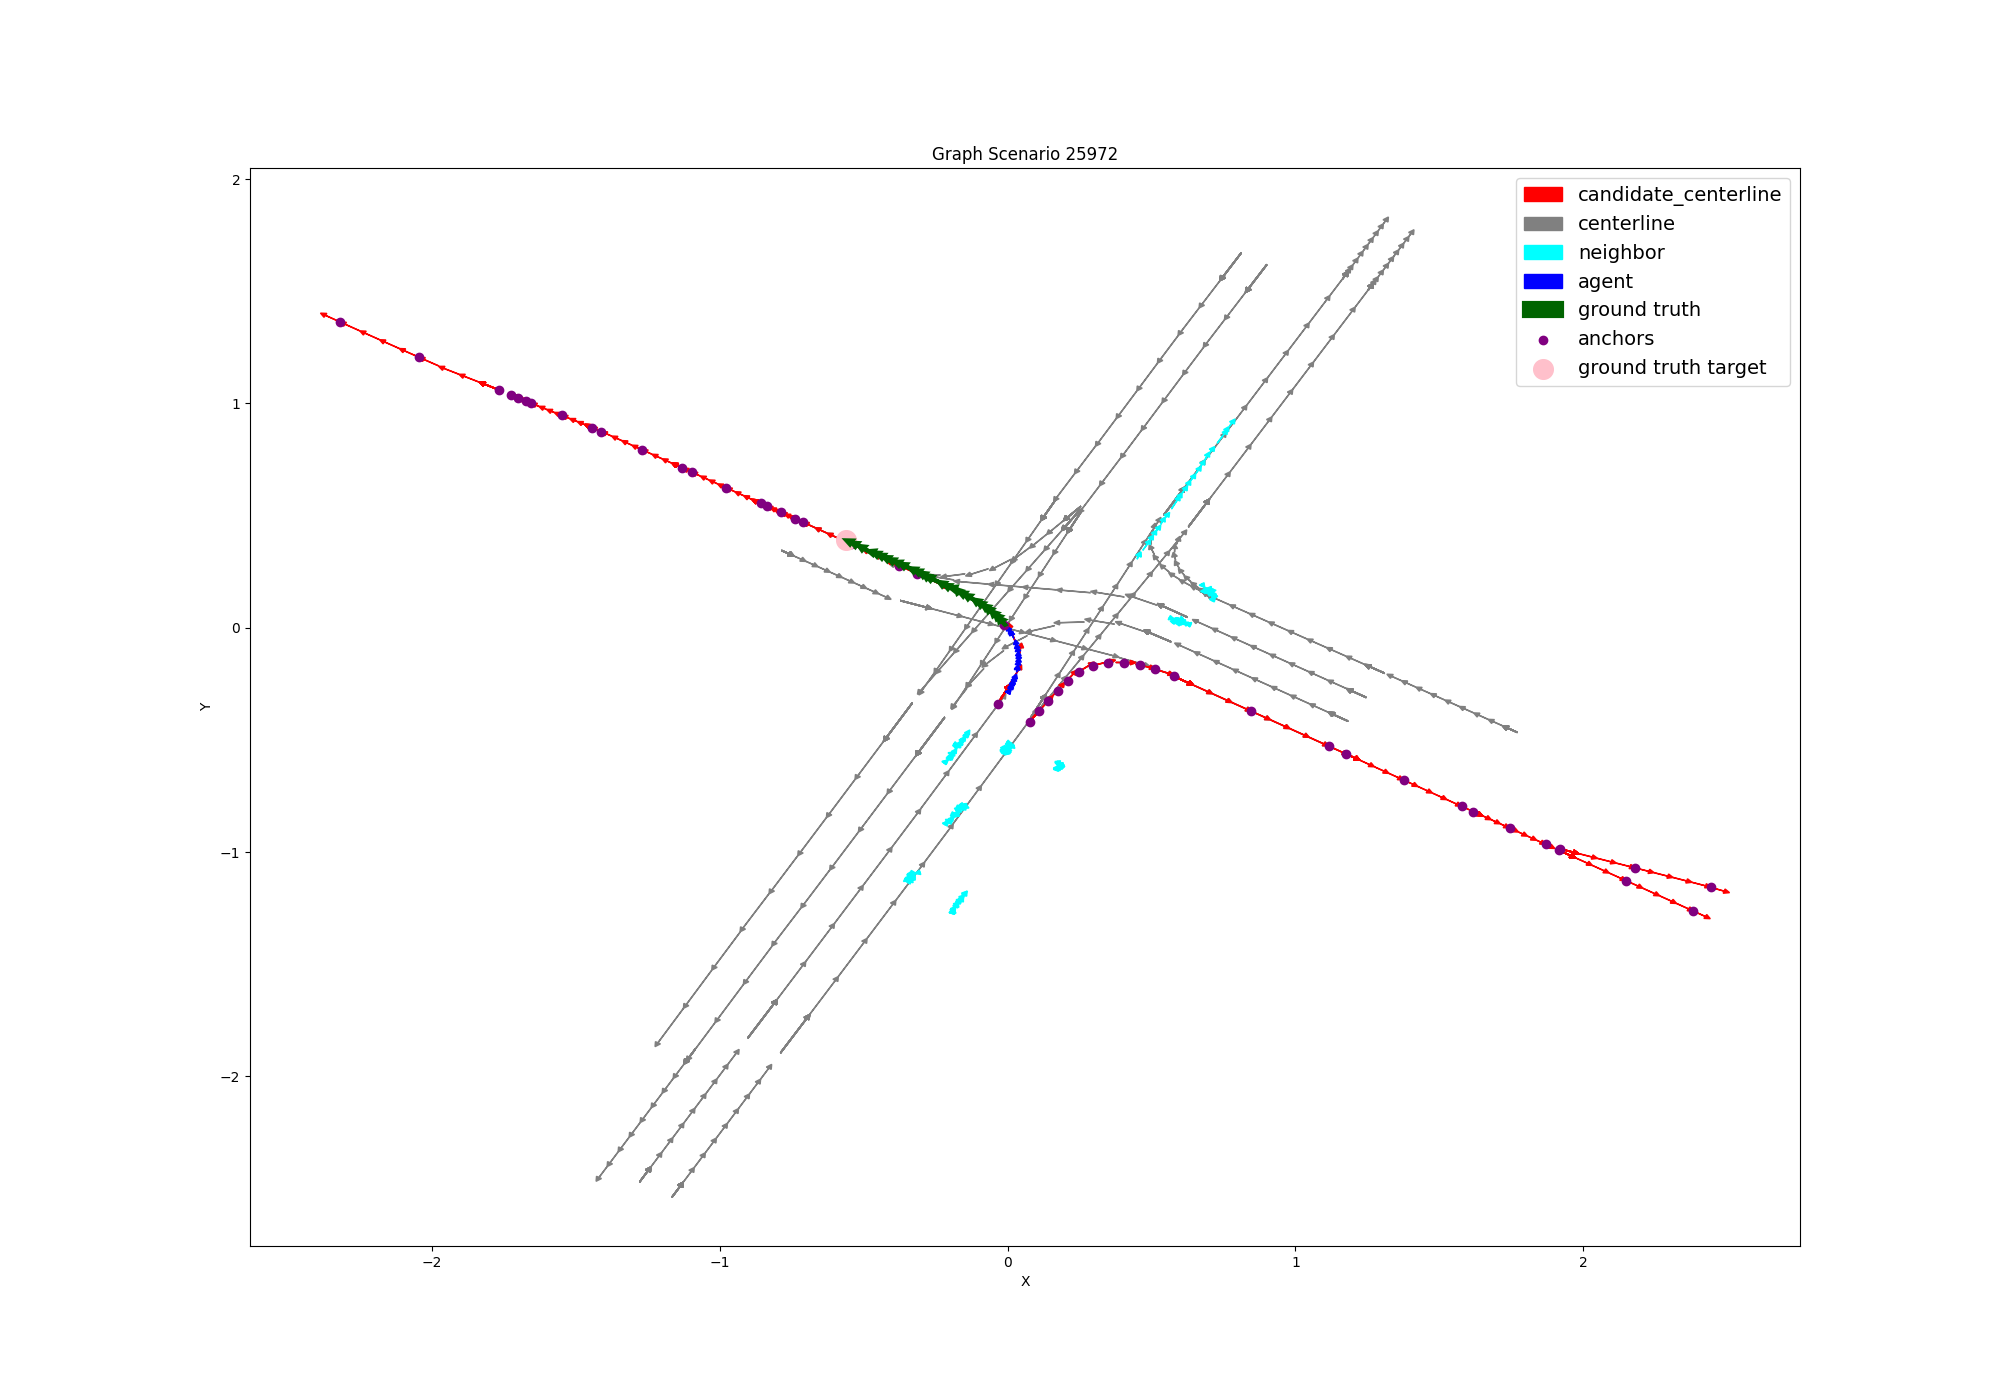
\includegraphics[width=1.0\textwidth]{images/polylines-representation.png}
  \caption{Визуализација репрезентације сложеним линијама}
  \label{polylines-representation}
\end{figure}

\section{Модел \textit{VectorNet}}

Као што је у уводном делу ове гране објашњено, сваку трајекторију и сегмент пута на сцени можемо да представимо сложеном линијом. Сваки
чвор сложене линија садржи издвојена својстава. \textit{VectorNet} је хијерархијска графовска неуронска мрежа која се састоји из три компоненте: \cite{vectornet}
\begin{itemize}
  \item Конструкција подграфа: Агрегација сложених линија у један вектор који се даље посматра као чвор у глобалном графу;
  \item Моделовање интеракција на високом нивоу у глобалном графу;
  \item Предикција трајекторија за чворове глобалног графа који одговарају агентима.
\end{itemize}

\subsection{Подграф}

Свака сложена линија на сцени се посматра као посебан граф. Применом варијанте графовске неуронске мреже
се издвајају битна својства и везе између чворова. Резултат се на крају агрегира како би се добио један вектор који представља репрезентацију

Архитектура подграфа је варијанта \textit{GCN} архитектуре \cite{gcn} са више слојева. Визуализација једног слоја се види на слици \ref{vectornet-subgraph}. 
Сваки слој може да се представи следећом формулом:

\begin{figure}[H]
  \centering
  $v^{(l+1)}_{i} = \rho_{rel}(g_{enc}(v^{(l)}_{i}),\ \rho_{agg}(A, \{g_{enc}(v^{(l)}_{j})\})))$
\end{figure}

Овде је $v^{(l)}_{i}$ вектор својства чвора из претходног слоја ($v^{(0)}_{i}$ су улазна својства), $g_{enc}$ слој за енкодирање својства чвора, 
$\rho_{agg}$ операција агрегације порука добијених од суседа, $A$ je матрица повезаности сложене линије, 
а $\rho_{rel}$ операција обједињавања агрегираних порука суседа и својства самог чвора. Избор операција је произвољан.

\noindent Конкретно: \cite{vectornet}
\begin{itemize}
  \item $g_{enc}$ је потпуно повезана неуронска мрежа;
  \item $\rho_{agg}$ је максимум свих порука од суседа (\textit{max pool});
  \item $\rho_{rel}$ је конкатенација својста чвора и агрегираних порука;
  \item \textit{A} је у оригиналном раду матрица повезаности потпуно повезаног графа. Алтернативе су повезаност једног чвора са следећим 
  или свим следећим у сложеној линији. 
\end{itemize}

\noindent Вектор сложене линије се добија агрегацијом добијеног графа последњег слоја (нпр. \textit{max pool}):

\begin{figure}[H]
  \centering
  $P_{feat} = \rho_{agg}(\{v^{(L)}_{i}\})$
\end{figure}

\begin{figure}[H]
  \centering
  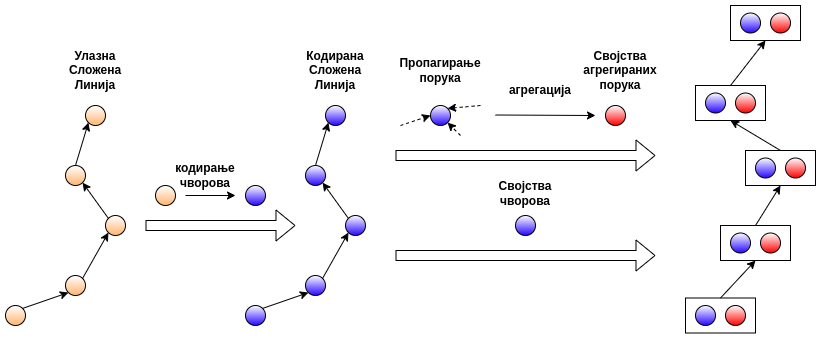
\includegraphics[width=0.9\textwidth]{images/vectornet-subgraph-rs.drawio.png}
  \caption{Визуализација једног слоја \label{vectornet-subgraph}}
\end{figure}

Из угла имплементације, улаз у ову компоненту је модела је вектор димензије $(B, P, T, F)$, где је $B$ димензија подскупа података једног корака, 
$P$ је број сложених линија у једном графу, $T$ је дужина сложене линије, a $F$ је број својстава. Након $L$ слојева се добија вектор димензије 
$(B, P, T, F \cdot 2^{L})$ који се агрегира на нивоу чворова на вектор димензије
$(B, P, F \cdot 2^{L})$\footnote{Претпоставка је да свака сложена линија има исти број својстава и да сваки граф има исти број сложених линија}. 
Агрегирану сложену линију посматрамо као један чвор у глобалном графу.
         
\subsection{Глобални граф интеракција}

Глобални граф интеракција се посматра као класичан граф са матрицом повезаности \textit{A} преко које може да се дефинише хеуристика, као што је на пример удаљеност
чворова на сцени. У оригиналном раду се ради једноставности глобални граф посматра као потпуно повезан граф без тежина. \cite{vectornet}

\begin{figure}[H]
  \centering
  $\{P^{(l+1)}_{i}\} = GNN(\{P^{(l)}_{i}\}, A)$
\end{figure}

\noindent Графовска неуронска мрежа је имплементирана као механизам пажње \cite{attention_is_all_you_need}:

\begin{figure}[H]
  \centering
  $GNN = softmax(\frac{P_{Q}P^{T}_{K}}{\sqrt{d_{K}}})P_{V}$
\end{figure}

Циљ ове компоненте је разумевање интеракција између агената и осталих објеката на сцени: који објекти у околини су у интересу, који путеви у околини су
у интересу, ...

\subsection{Предикција трајекторија}

За предикцију трајекторија се филтрирају чворови агената из глобалног графа интеракције. За сваког агента се примењује призвољан \textit{decoder} модел
чији је излаз предикција трајекторије. Наједноставнији приступ је коришћење потпуно повезане неуронске мреже под претпоставком да су 
тачке трајекторије међусобно независне. Овај корак се замењује напреднијим приступоп у модификованој верзији описаној у следећој секцији.

\subsection{Функција грешке}

За функцију грешке предикције трајекторија $L_{traj}$ се користи \textit{huber} функција грешке тј. комбинација \textit{L1} и \textit{L2} функције грешке. У процесу
тренирања може да се дода задатак \textbf{естимације недостајућих чворова глобалног графа интеракција}. Насумично се бирају чворови у графу и замаскирају
се његова својства (множењем са нулом). Сваком чвору се додају две ,,нове`` вредности које су једнаке минималној вредности свакој од координата почетних 
тачака сложене линије\footnote{Опис својстава сложених линија је описан у секцији за припрему података}. Нове вредности представљају идентификаторе
тих сложених линија који се користе приликом тренирања модела за естимацију недостајућих својстава чворова. Циљ овог задатка је форсирање бољег разумевања
веза између трајекторија и генерално веза између сложених линија у графу. Функцију грешке овог задатка ($L_{node}$) се имплементира коришћењем \textit{L1}
функција грешке. \cite{vectornet} 

\begin{figure}[H]
  \centering
  $L = L_{traj} + \alpha \cdot L_{node}$
\end{figure}

\section{Модификована верзија \textit{VectorNet} са узоркованим крајњим тачкама трајекторија}

Претходно поменута верзија \textit{VectorNet} модела може да се унапреди додавањем доменског знања. Један приступ је да се користе унапред
дефинисани предлози трајекторија који се користе као основе за генерисање предикција трајекторија. Предлози се бирају на основу 
анализе података (кластеровање). \cite{multipath}
Ова метода је аналогна примени предлога (,,сидра`` - \textit{eng. anchors}) која се користи у детекцији објеката.

Алтернатива која се исто заснива на предлозима (,,сидрима``) је да уместо предлога трајекторија користе предлози крајњих тачака трајекторија. Модел
који генерише трајекторију на основу крајње тачке и својства из \textit{VectorNet} се лако тренира, али квалитет целог система доста зависи
од квалитета узорковања тих предлога. 

Архитектура \textit{tnt: Target-driveN Trajectory Prediction} \cite{tnt} се заснива баш на тој идеји. Кораци:
\begin{enumerate}
  \item Разумевање контекста помогућу \textit{VectorNet} модела (основа);
  \item Генерисање корекција и поузданости за сваки предлог крајње тачке трајекторије;
  \item Узорковање модификованих предлога на основу поузданости;
  \item Естимација трајекторије до сваког изабраног предлога крајње тачке.
  \item Естимација вероватноћа за сваку од добијених трајекторија;
  \item Филтрирање трајекторија на основу вероватноћа.
\end{enumerate}

Уместо последња два корака могу да се користе вероватноће (поузданости) предлога крајњих тачака, али из добре крајње тачке не следи
нужно да је добијена трајекторија такође квалитетна (нпр. уколико предложена трајектрорија прелази преко тротоара). 

Овде \textit{VectorNet} чини језгро архитектуре, а сви наредни кораци могу да се имплементирају потпуно повезаним неуронским мрежама уз комбинацију
једноставних детерминистичких алгоритама. Главни изазов ове архитектуре је у алгоритму за генерисање предлога
\footnote{Алгоритам је укратко описан у секцији за иницијалну припрему података} и балансирању
параметара функција грешака приликом учења модела.

\noindent Ако се не учи \textit{естимације недостајућих чворова глобалног графа интеракција} уз \textit{VectorNet}, 
онда функција грешке има следећи облик:

\begin{figure}[H]
  \centering
  $L = \lambda_{1} \cdot L_{offsets} + \lambda_{2} \cdot L_{tarconf} + \lambda_{3} \cdot L_{trajde} + \lambda_{4} \cdot L_{trajconf}$
\end{figure}

Нека је $P_{anchors}$ скуп свих предлога крајњих тачака трајекторија и нека је $P_{gt}$ истинита крајња тачка трајекторије. Тада се изваја
из скупа $P_{anchors}$ елемент $P_{closest}$ који је најближи истинитој крајњој тачки\footnote{Овде не узимамо у обзир поправке, 
већ нетрансформисане, узорковане вредности. 
Уколико се у обзир узимају вредности са поправкама, онда процес учења постаје тежак због шума (мења се индекс најближе тачке). Ово можда не би био
толики проблем да су остале трајекторије другачије дефинисане тј. независне од промене изабране, најближе тачке.}. 
Тада је:

\begin{figure}[H]
  \centering
  $L_{offsets} = H_{delta}(P_{closest\_offset}, \hat{P}_{closest\_offset})$
\end{figure}

\noindent где је $H_{delta}$ \textit{huber} функција грешке са параметром \textit{delta}, $P_{closest\_offset} := P_{gt} - P_{closest}$,
а $\hat{P}_{closest\_offset}$ је предикција тог одступања. Циљ је да баш тај најближи предлог има највећу поузданост, па се функција грешке за 
поузданост дефинише на следећи начих:

\begin{figure}[H]
  \centering
  $L_{tarconf} = BCE(P_{closest\_onehot}, \hat{P}_{confs})$
\end{figure}

\noindent где \textit{BCE} је бинарна унакрсна ентропија, $P_{closest\_onehot}$ индекс елемента $P_{closest}$ у \textit{onehot} 
формату\footnote{Индекс се представља као низ димензије броја класа (предложених крајњих тачака у овом случају) где су свуда нуле сем на локацији која одговара
вредности тог индекса.} и $\hat{P}_{confs}$ поузданост модела за сваки предлог (за сваки предлог се даје поузданост из интервала $[0, 1]$). Функција грешке за
трајекторије је аналогна као и за предлога крајњих тачака. Састоји се из функције грешке за одступање трајекторија од реализације и оцене
поузданости модела за сваку од тих трајекторија.

\begin{figure}[H]
  \centering
  $L_{trajde} = H_{delta} (T_{traj}, \hat{T}_{traj})$
\end{figure}

\noindent где је $T_{traj}$ истинита вредност трајекторије, а $\hat{T}_{traj}$ је њена предикција. Приликом учења се за естимацију трајекторије 
$\hat{T}_{traj}$ узима истинита крајња тачка трајекторије како би учење било стабилније. Ова техника се зове ,,Учитељско форсирање`` \cite{teacher_forcing}.
Последња компонента се односи на поузданост модела за сваку естимацију трајекторија. За сваку естимирану трајекторију се рачуна максимално растојање 
између свих упарених тачака естимиране трајекторије и истините вредности трајекторије тј. 
$D(T_{traj}, \hat{T}_{raj}) := max(||T^{k}_{traj} - \hat{T}^{k}_{traj}||^{2}_{2})$. Тада се ,,истинита расподела`` $P_{traj\_confs}$ одређује као \textit{softmax} 
ових негативних вредности.

\begin{figure}[H]
  \centering
  $L_{trajconf} = BCE(P_{traj\_confs}, \hat{P}_{traj\_confs})$
\end{figure}

\section{Припрема података}

Припрема података у овој секцији се наставља на иницијални процес претпроцесирања података и своди се на трансформацију свих елемената
\textit{HD} мапа у сложене линије. Да би било могуће спојити више сценарија у један подскуп података за једну итерацију тренирања, неопходно
је да се испуне одређена ограничења:
\begin{itemize}
  \item Сваки сценарио мора да има исти број сложених линија ($N_{p}$). Ако је број сложених линија већи од $N_{p}$, онда се 
        вишак сложених линија одбацује, при чему се води рачуна о приоритету сложеих линија: агент, остали објекти, путеви, путеви кандидати.
        Ако је број сложених линија мањи од $N_{p}$, онда се скуп допуњава сложеним линијама са нула чворовима.
  \item Свака сложена линија мора да има исти број чворова ($N_{n}$). Ово се решава аналогно броју сложених линија.
  \item Сваки чвор сложених линија мора да има исти број својстава ($N_{f}$). Сваки чвор има иста својства, са тим
        да се својства допуњавају нулама ако немају смисла за тај тим сложених линија (агент и путеви немају иста својства).
\end{itemize}

\noindent Сваки чвор сложене линије има следећа својства:
\begin{itemize}
  \item Координате \textit{x} и \textit{y}: Просек претходне и тренутне тачке трајекторије - 2 скалара;
  \item Смер по \textit{x} и \textit{y}: Разлика тренутне и претходне тачке трајекторије - 2 скалара;
  \item Тип објекта као \textit{onehot} вектор (агент, сусед - објекат, пут, пут кандидат) - 4 скалара;
  \item Метаподаци путних чворова (нуле у случају трајекторија агента и објеката суседа)
    \begin{itemize}
      \item Да ли се сегмент пресеца са неким другим сегментом - 1 скалар;
      \item Да ли постоји контрола саобраћаја - 1 скалар;
      \item Смер као \textit{onehot} вектор (нема, десно, лево) - 3 скалара
    \end{itemize}
  \item Да ли је чвор прави (1) или вештачки (0) - 1 скалар.
\end{itemize}

Коначан формат улазних података у \textit{VectorNet} је $(B, N_{p}, N_{n}, 14)$, где је $B$ број сценарија у једном подскупу података,
а $N_{p}$ и $N_{n}$ су параметри.

\section{Експерименти и резултати}

\begin{figure}[H]
  \centering
  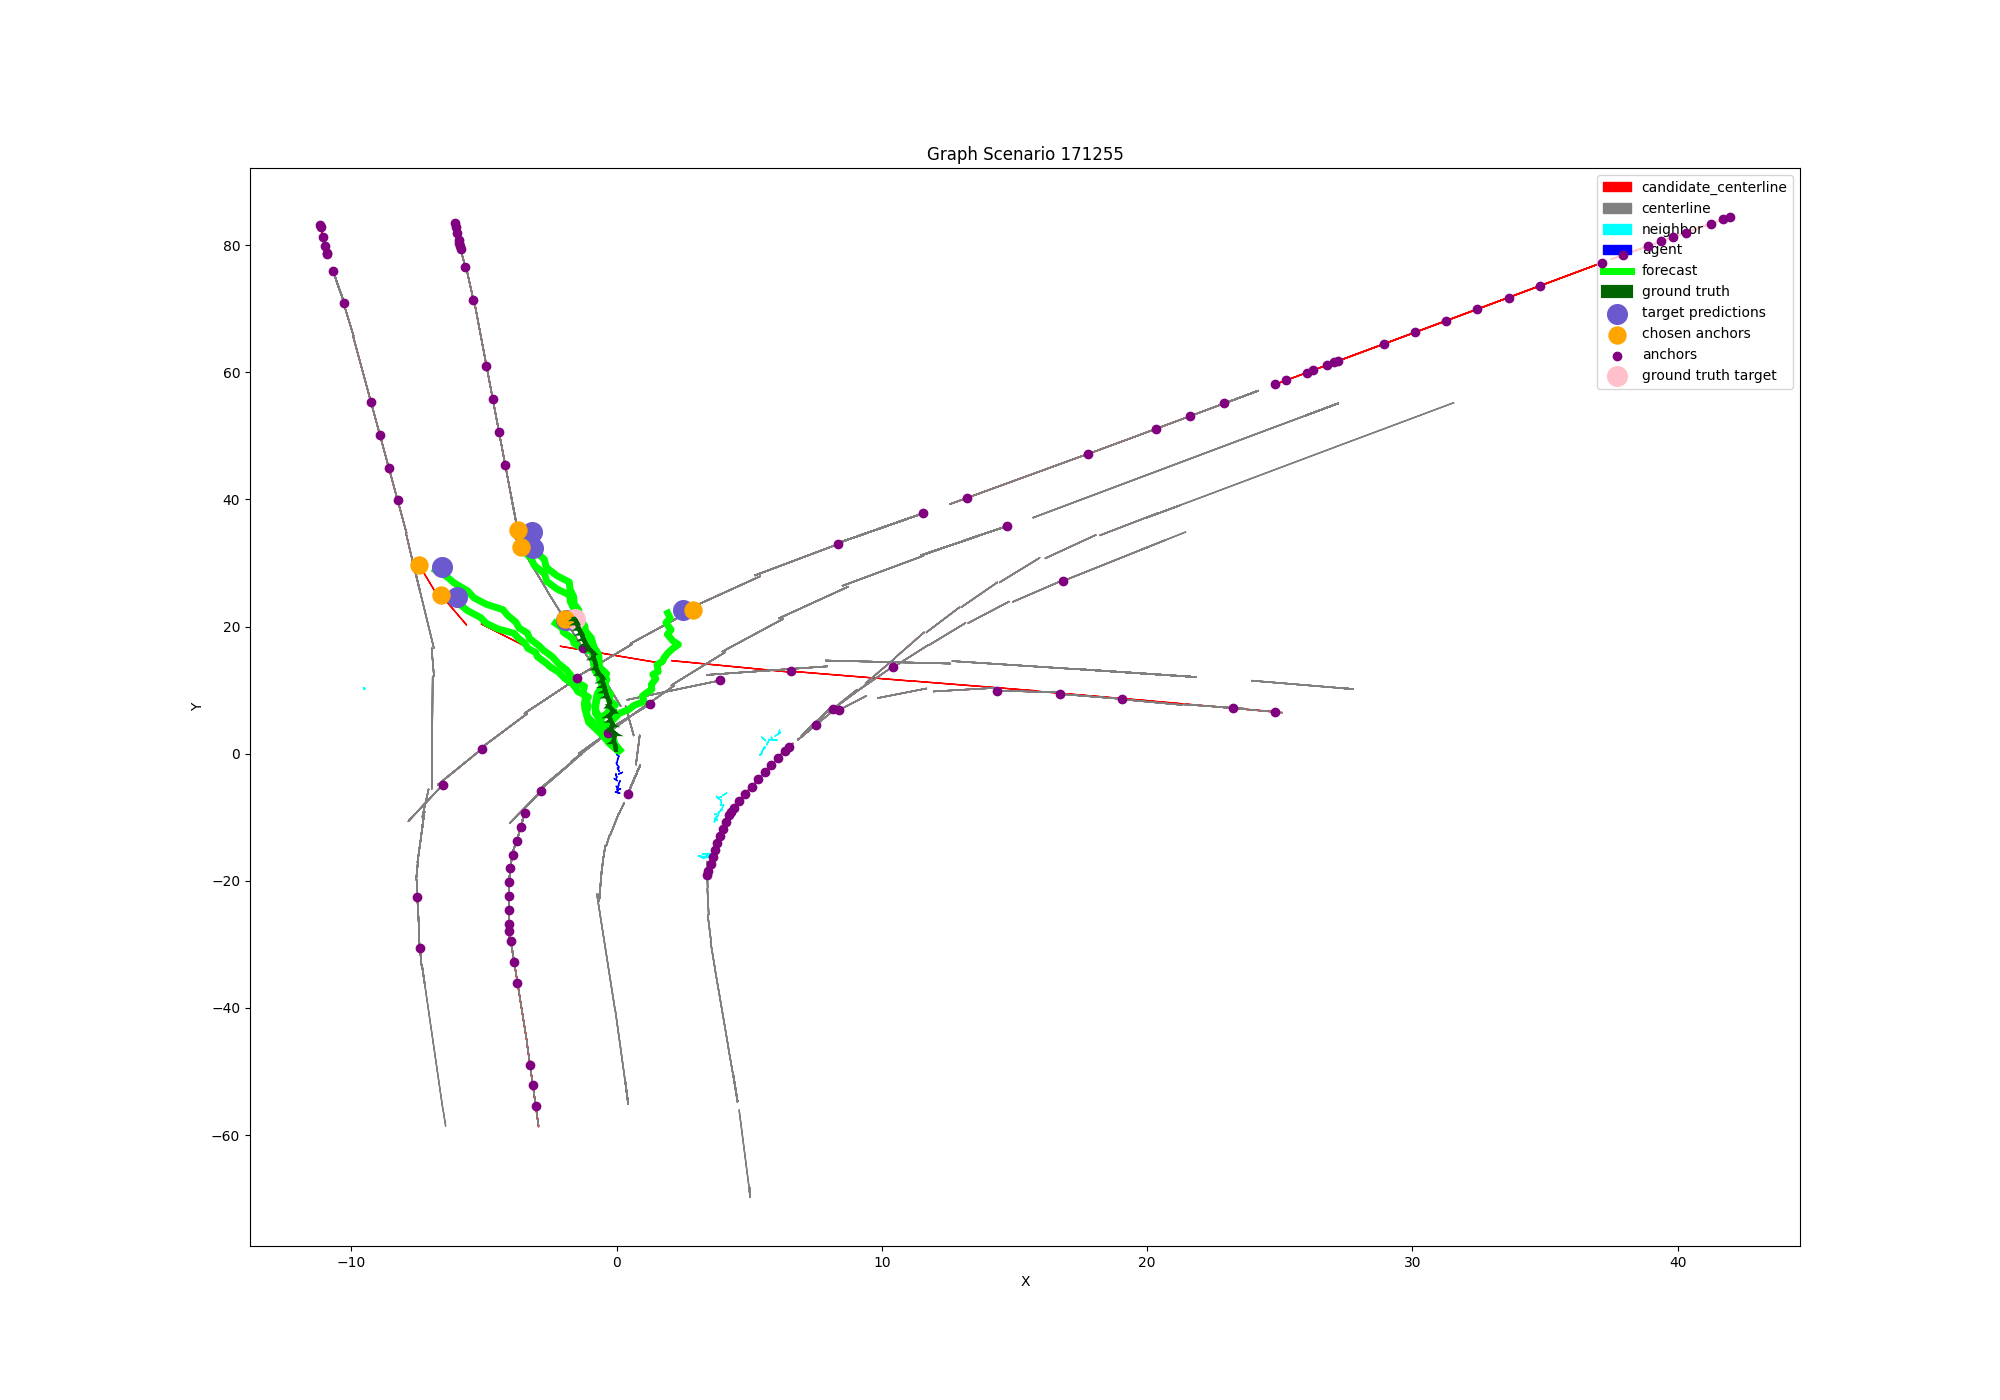
\includegraphics[width=0.9\textwidth]{images/tnt-scenario-171255.png}
  \caption{
    Пример резултата за сценарио 171255 - $minADE_{6} = 0.6, minFDE_{6} = 1.0$. Сивом 
    бојом су обојени путеви, тамно плавом је обојена историја трајекторија агента, светло плавом су обојене историје суседних објеката,
    црвеном линијом су обојени путеви кандидати. Мали љубичасти кругови су узорковани предлози, велики плави кругови су изабрани
    узорковани предлози са највећом поузданошћу, а велики наранџасти кругови су модификовани изабрани предлози. Светло зеленом
    бојом су представљене предикције за сваку од изабраних крајњих тачака, а тамно зеленом бојом су обојени истинити резултати. 
    \label{tnt-scenario-171255}
  }
\end{figure}

На слици \ref{tnt-scenario-171255} је приказан пример примене \textit{TNT-VectorNet} архитектуре. 

% ------------------------------------------------------------------------------
\chapter{Техника заснована на разумевању контекста обрадом растеризоване сцене}
\label{chp:razrada}
% ------------------------------------------------------------------------------

TODO: За овај део бих као енкодер такође користио VectorNet уместо растеризоване сцене уз растеризоване топлотне мапе. 

% ------------------------------------------------------------------------------
\chapter{Закључак}
% ------------------------------------------------------------------------------
У изради...

% ==============================================================================
% Završni deo teze i prilozi
\backmatter
% ==============================================================================

% Datoteka sa literaturom u BibTex tj. BibLaTeX/Biber formatu
\bibliography{matfmaster-primer}
\bibliographystyle{ieeetr}

% ------------------------------------------------------------------------------
% Biografija kandidata
\begin{biografija}
\textbf{Момир Аџемовић} 
У изради...
\end{biografija}
% ------------------------------------------------------------------------------

\end{document} 